\subsubsection{要件定義}
本システムはサーバ,クライアントで以下の要件を持たす必要がある.

まずサーバの要件を示す.

\begin{itemize}
    \item Dockerの動作: すべての開発にDockerを用いる
    \item Webサーバの動作: Webアプリケーションの公開に用いる
    \item Pythonの動作: Djangoの動作に用いる
    \item Goの動作: APIの動作に用いる
    \item PostgreSQLの動作: ユーザの管理等のデータベースとして用いる
\end{itemize}

サーバはWebサーバを用いてクライアントをネットワークに公開し,Dockerを用いてPythonとGoとPostgreSQLを動作させる.
PythonはDjangoを動作させ,クライアントにGUI等を提供する.
GoはAPI作成に用いて,Dockerを操作する.
PostgreSQLは,Djangoを通してクライアントから入力されたデータ等を保存する.

続いて,クライアントの要件を示す.

\begin{itemize}
    \item html5が解釈できるWebブラウザの動作: クライアントの動作環境となる 
\end{itemize}

クライアントはWebアプリケーションであり,html5で記述されている.
クライアントは教材提供者と学習者に対してGUIを提供する.
詳細は,\ref{sec:fun1}節,\ref{sec:fun2}節,\ref{sec:fun3}節で述べる.

\newpage
\subsubsection{システム構成}
本システムの構成を図\ref{system}に示す.本システムはDjangoで構成されるアプリケーション部(以下,クライアント),およびGoとdjangorestframeworkで構成されるサーバ部(以下,サーバ)から構築される.
サーバはAPIを用いて統計情報提供機能とコンテナ管理機能を動作させる.

\begin{figure}[htbp]
    \begin{center}
        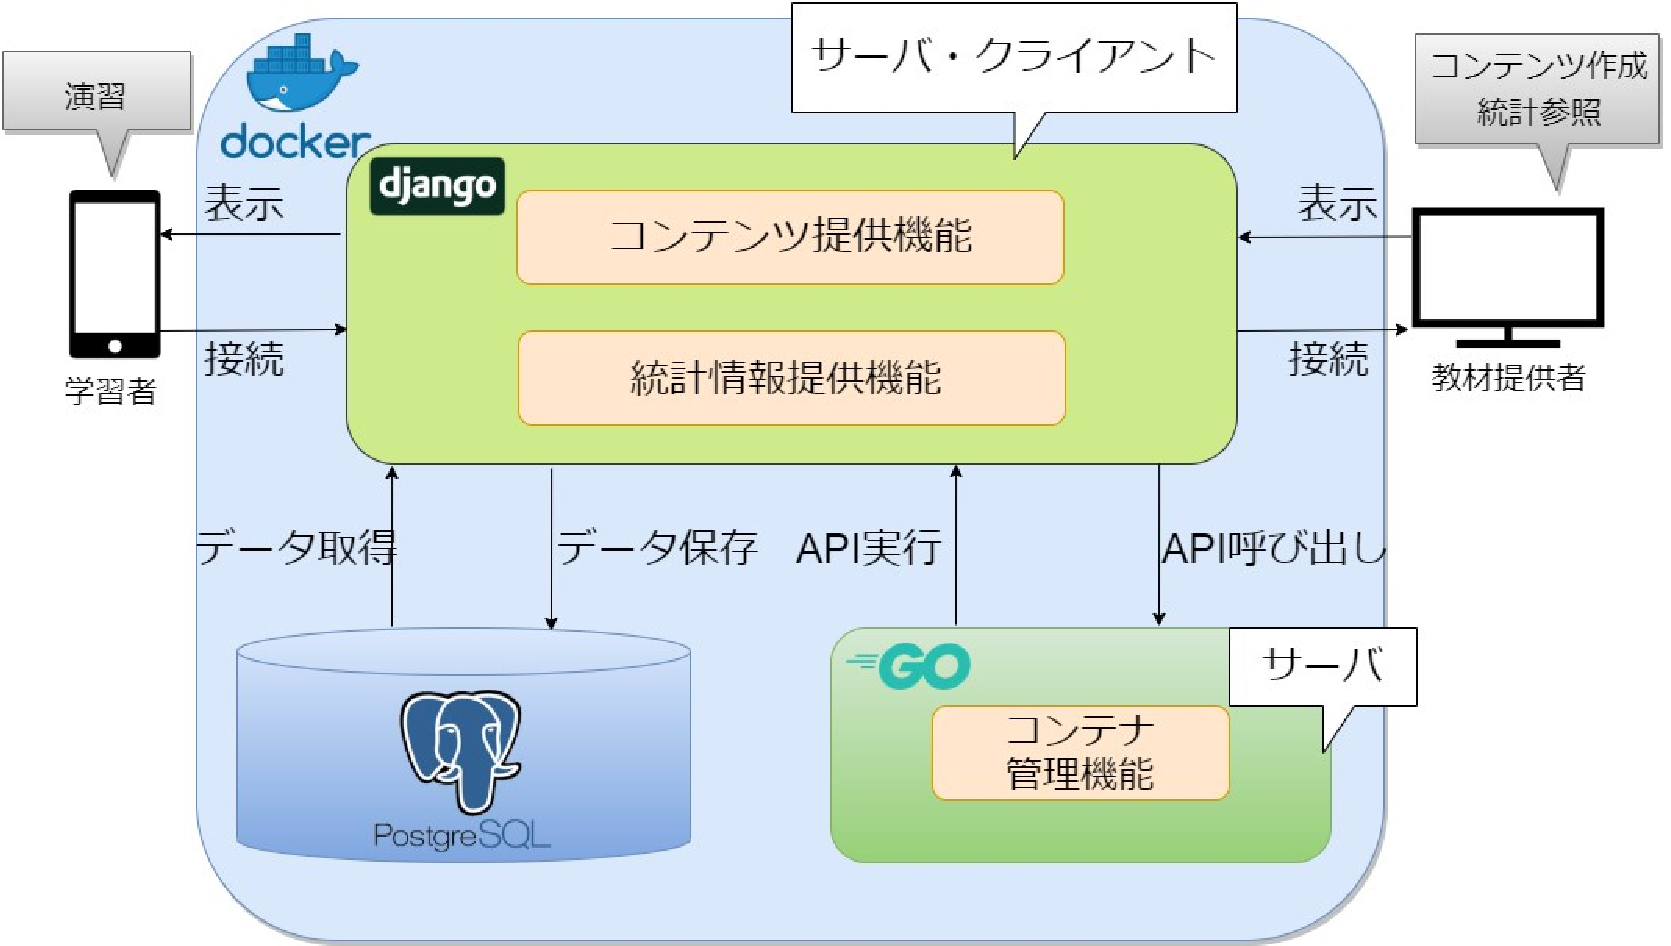
\includegraphics[width=18cm,height=17cm,keepaspectratio]{system-crop.pdf}\\
        %includegraphicsの詳しい使い方ははLaTeXの参考書を参照.
    \end{center}
    \caption{システム構成}
    \label{system}
\end{figure}


コンテンツ提供機能のGUIを図\ref{teikyou}に,統計情報提供機能のGUIを図\ref{toukei}に,コンテナ管理機能のGUIを図\ref{kanri}にそれぞれ示す.

\newpage
教材提供者は図\ref{teikyou}のコンテンツ提供機能を用いて情報倫理に関するコンテンツを提供する.

\begin{figure}[htbp]
    \begin{center}
        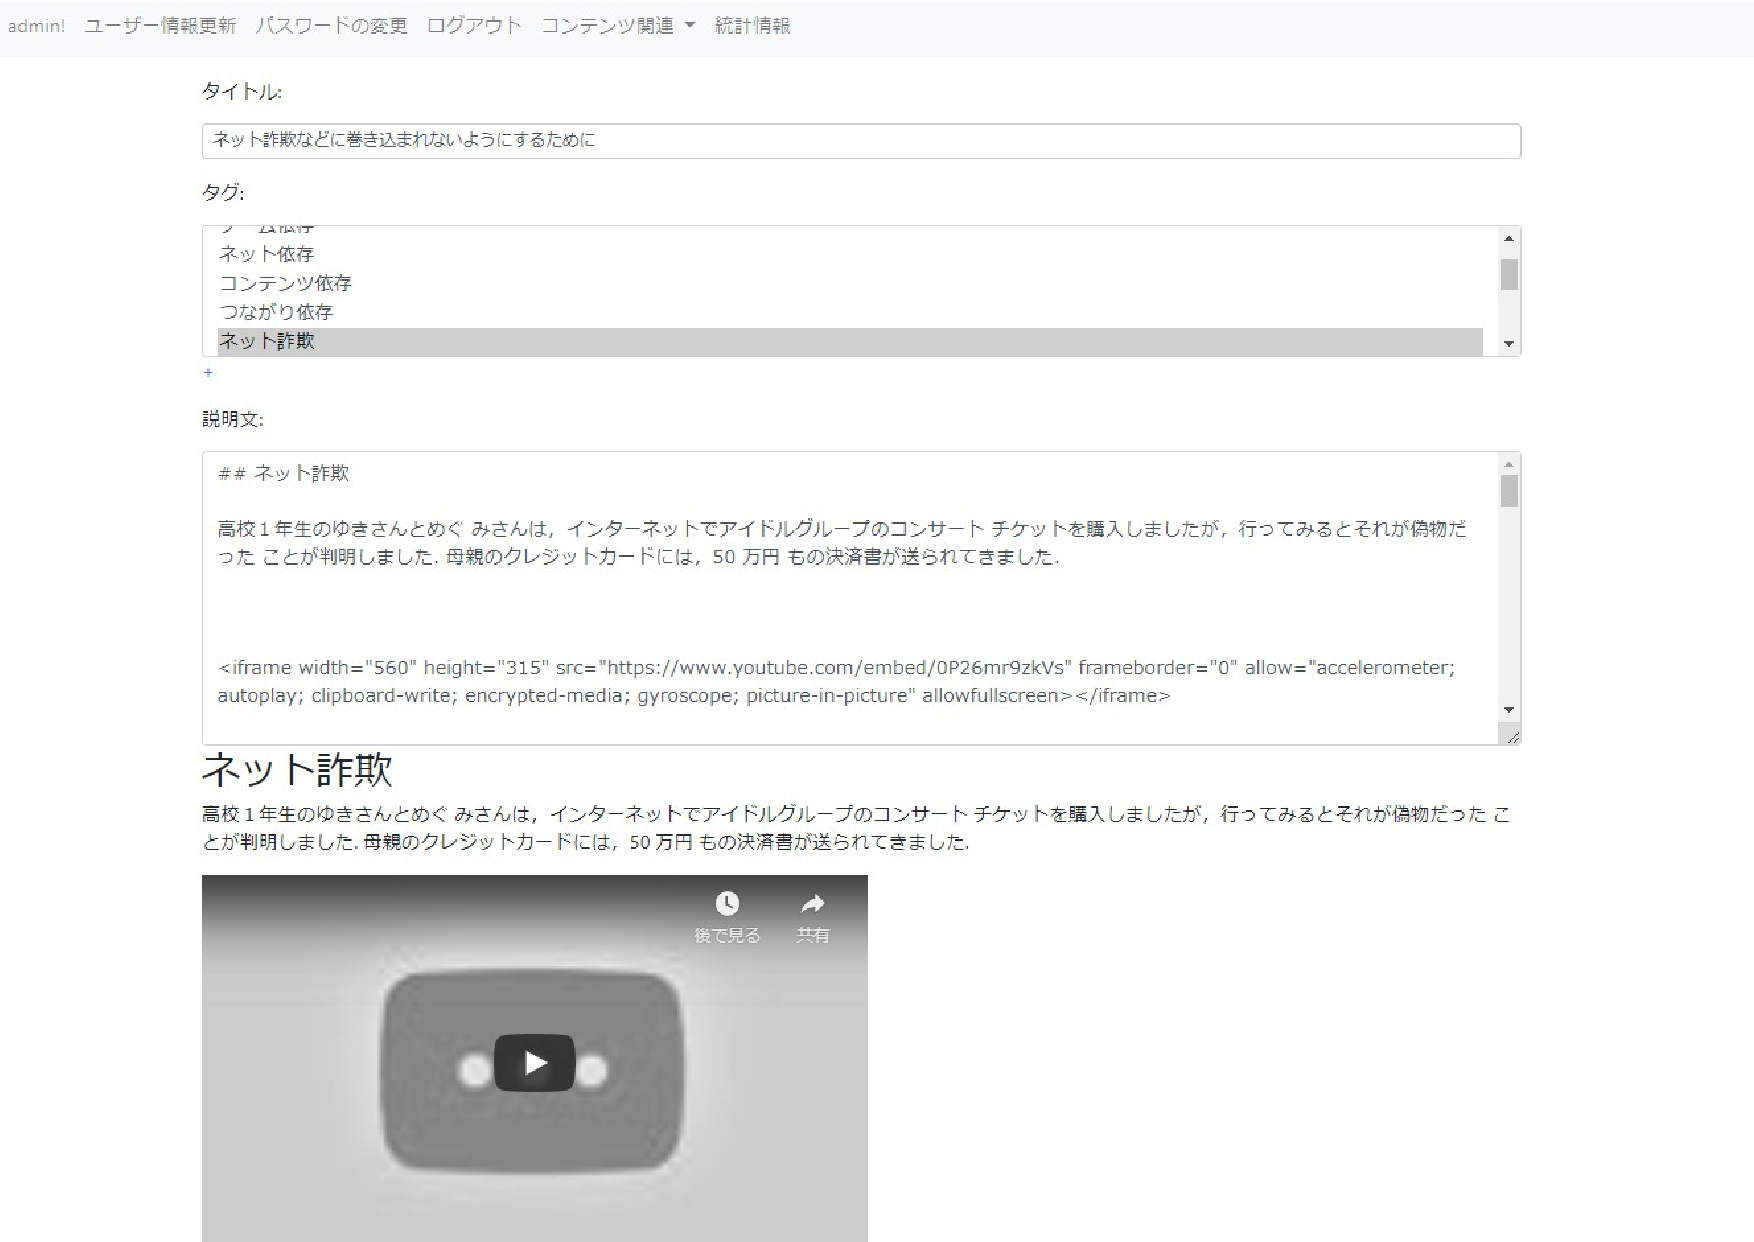
\includegraphics[width=18cm,height=17cm,keepaspectratio]{create_content-crop.pdf}\\
        %includegraphicsの詳しい使い方ははLaTeXの参考書を参照.
    \end{center}
    \caption{コンテンツ提供機能のGUI}
    \label{teikyou}
\end{figure}

\newpage
図\ref{toukei}の統計情報提供機能では,教材提供者が学習者の回答情報等をグラフとして確認できる.
\begin{figure}[htbp]
    \begin{center}
        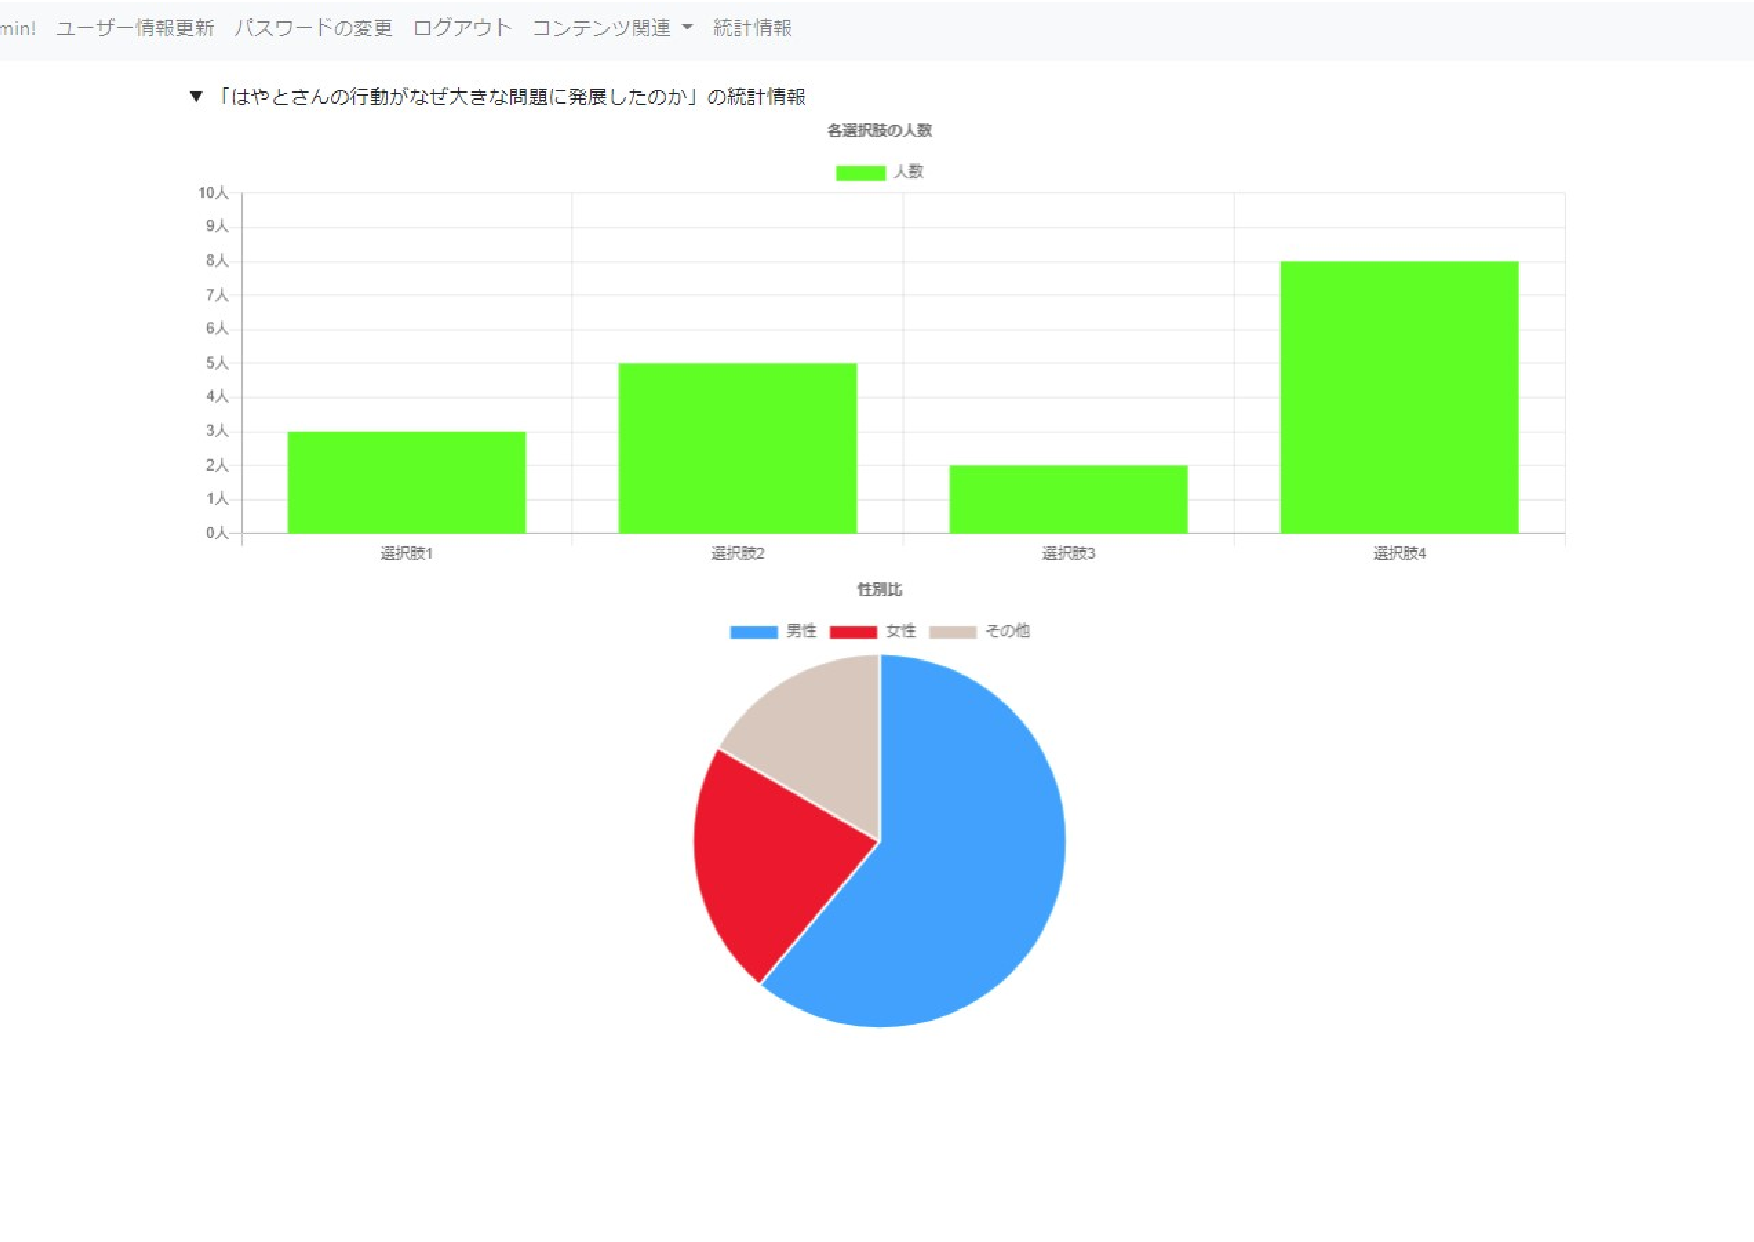
\includegraphics[width=18cm,height=17cm,keepaspectratio]{toukei-crop.pdf}\\
        %includegraphicsの詳しい使い方ははLaTeXの参考書を参照.
    \end{center}
    \caption{統計情報提供機能のGUI}
    \label{toukei}
\end{figure}

\newpage
図\ref{kanri}のコンテナ管理機能では教材提供者がDockerを用いて作成した他の教育アプリケーションを本プラットフォームでも利用することが可能となる.
\begin{figure}[htbp]
    \begin{center}
        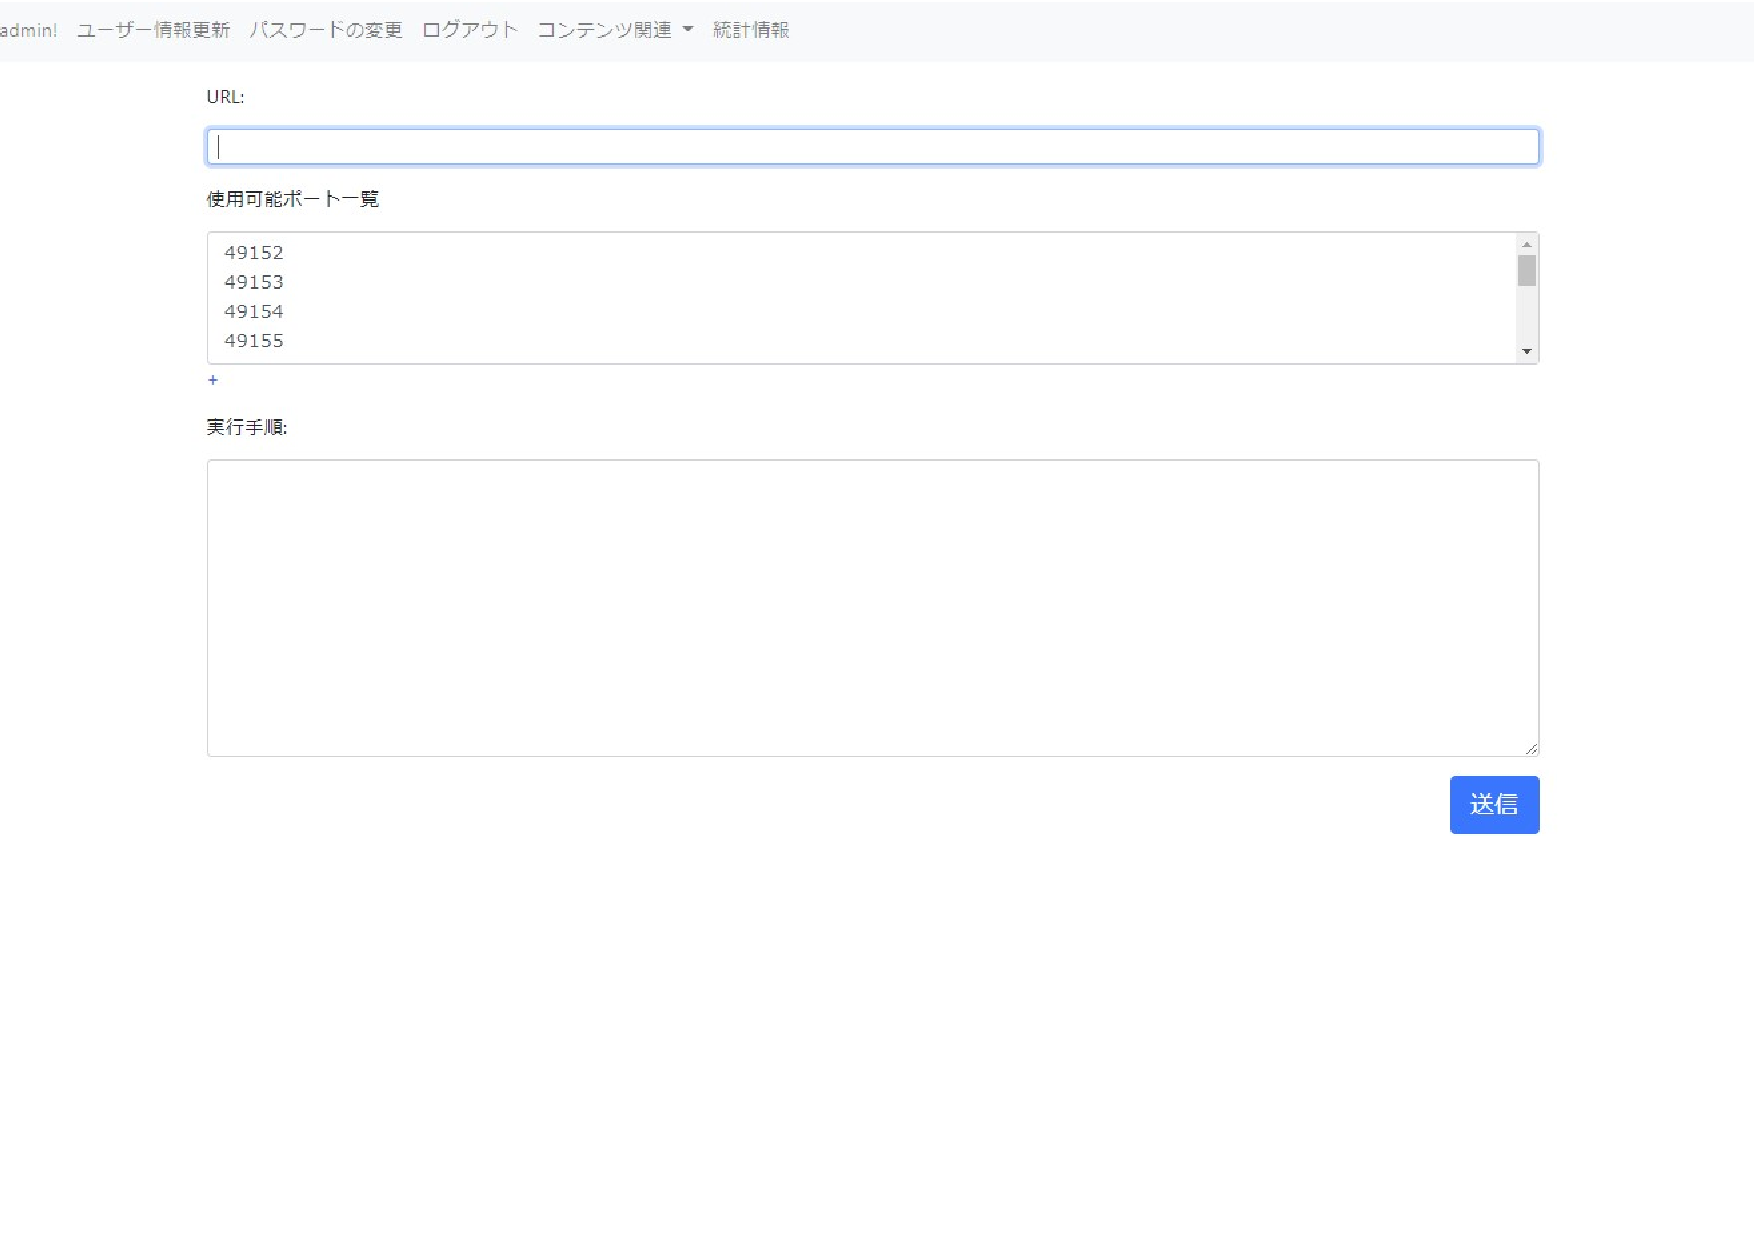
\includegraphics[width=18cm,height=17cm,keepaspectratio]{container_management-crop.pdf}\\
        %includegraphicsの詳しい使い方ははLaTeXの参考書を参照.
    \end{center}
    \caption{コンテナ管理機能のGUI}
    \label{kanri}
\end{figure}

\newpage
学習者は図\ref{teikyou}のコンテンツ提供機能を用いて作成されたコンテンツを図\ref{naiyou}のようにして閲覧,学習することが可能である.
\begin{figure}[htbp]
    \begin{center}
        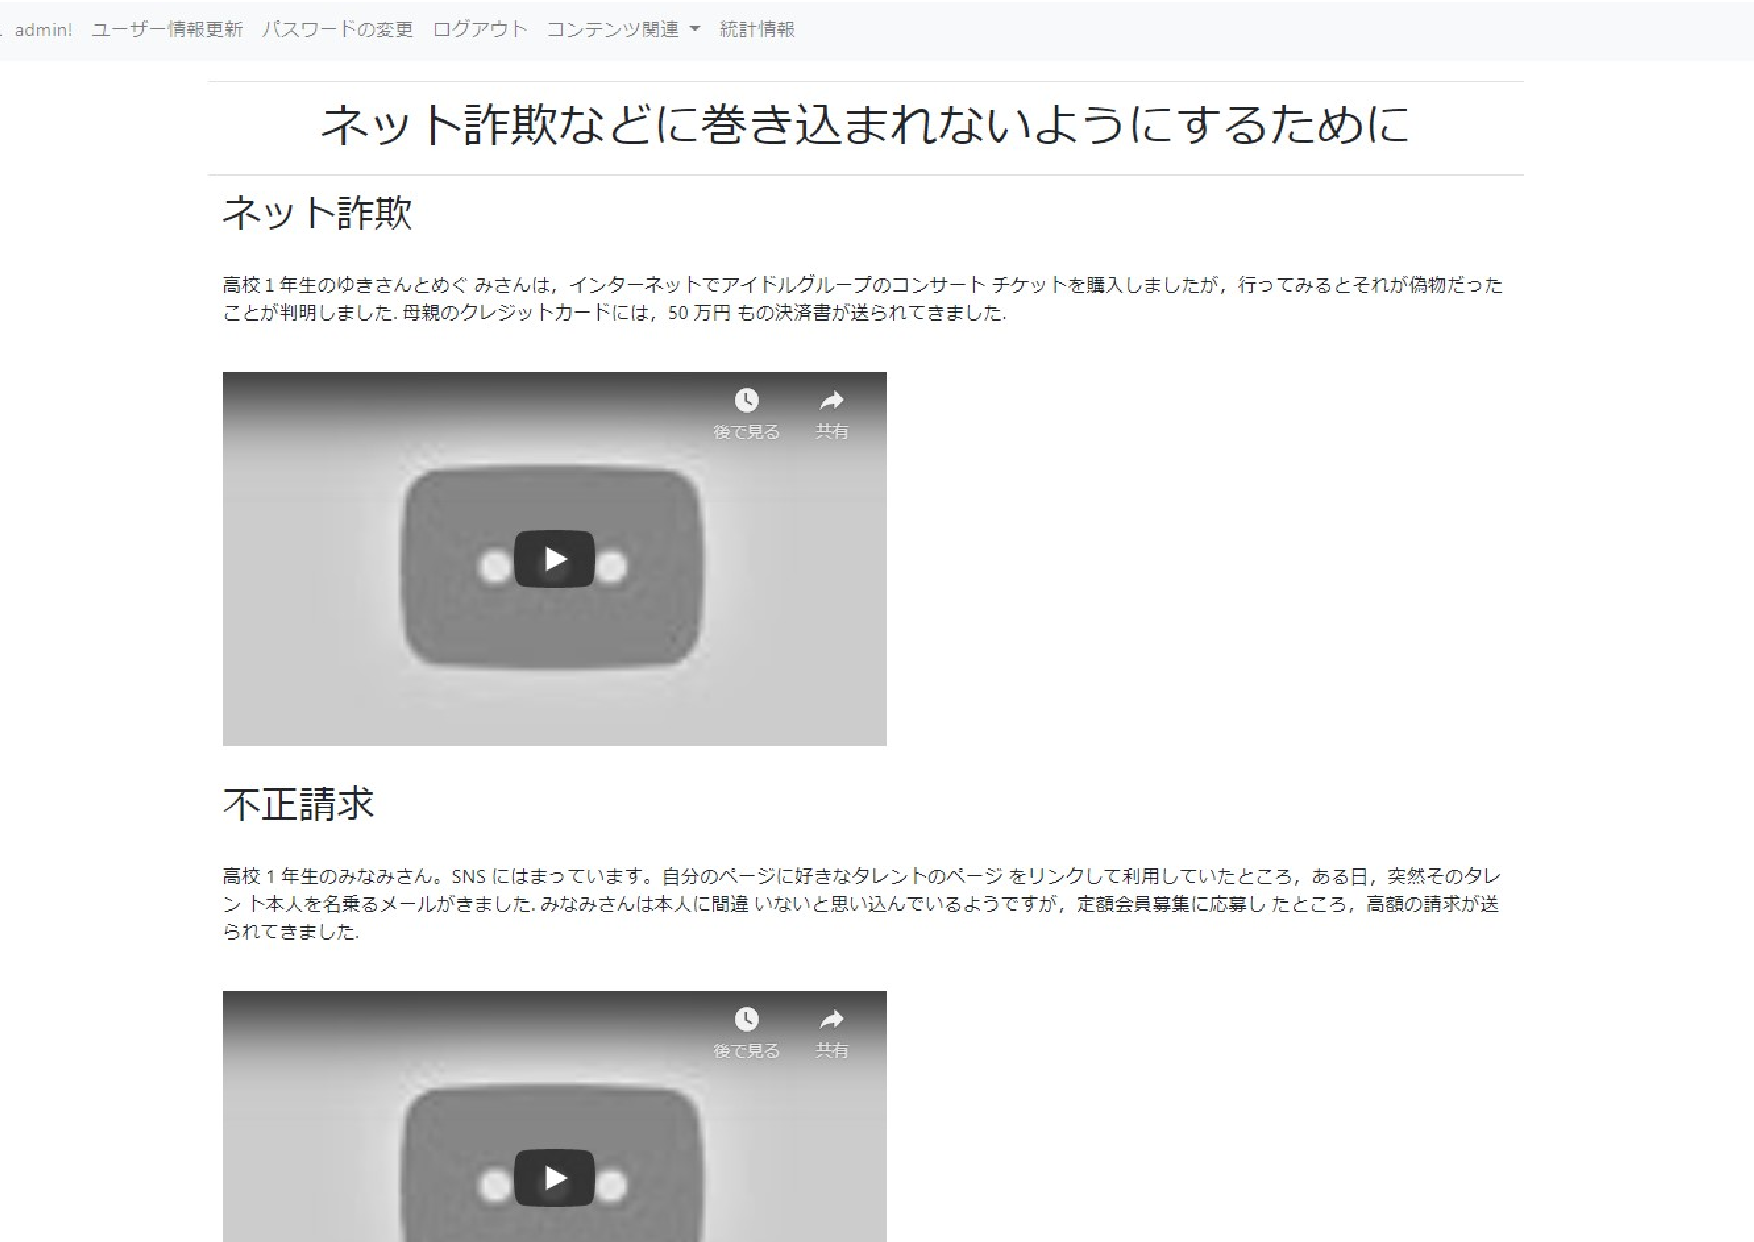
\includegraphics[width=18cm,height=17cm,keepaspectratio]{naiyou-crop.pdf}\\
        %includegraphicsの詳しい使い方ははLaTeXの参考書を参照.
    \end{center}
    \caption{コンテンツ閲覧時のGUI}
    \label{naiyou}
\end{figure}

\newpage
\subsubsection{システムの内部構成}
クライアントの内部構成を図\ref{client_naibu}に示す.はじめに,教材提供者および学習者が各々ネットワークに接続できる環境を用意し,Webブラウザを立ち上げ,特定のIPアドレスを入力しログインする.
ただし,教材提供者が本プラットフォームの機能を利用するにはログインは必須であるが,学習者は必須ではない.

Webブラウザで本プラットフォームに接続しログインした後,教材提供者はGUIのコンテンツ提供機能,統計情報提供機能,コンテナ管理機能を使用できる.
コンテンツ提供機能は教材提供者が入力した内容をサーバを介しデータベースに保存する.
統計情報提供機能はデータベースからサーバを介しデータを取得しWebブラウザ上に情報を表示する.
コンテナ管理機能は教材提供者が入力した内容をGoで作成したAPIで実行し,Dockerのコマンドを用いてコンテナが建ち上がっていることを確認し,建ち上がっていた場合それにアクセスするURLを画面上に発行する.

\begin{figure}[htbp]
    \begin{center}
        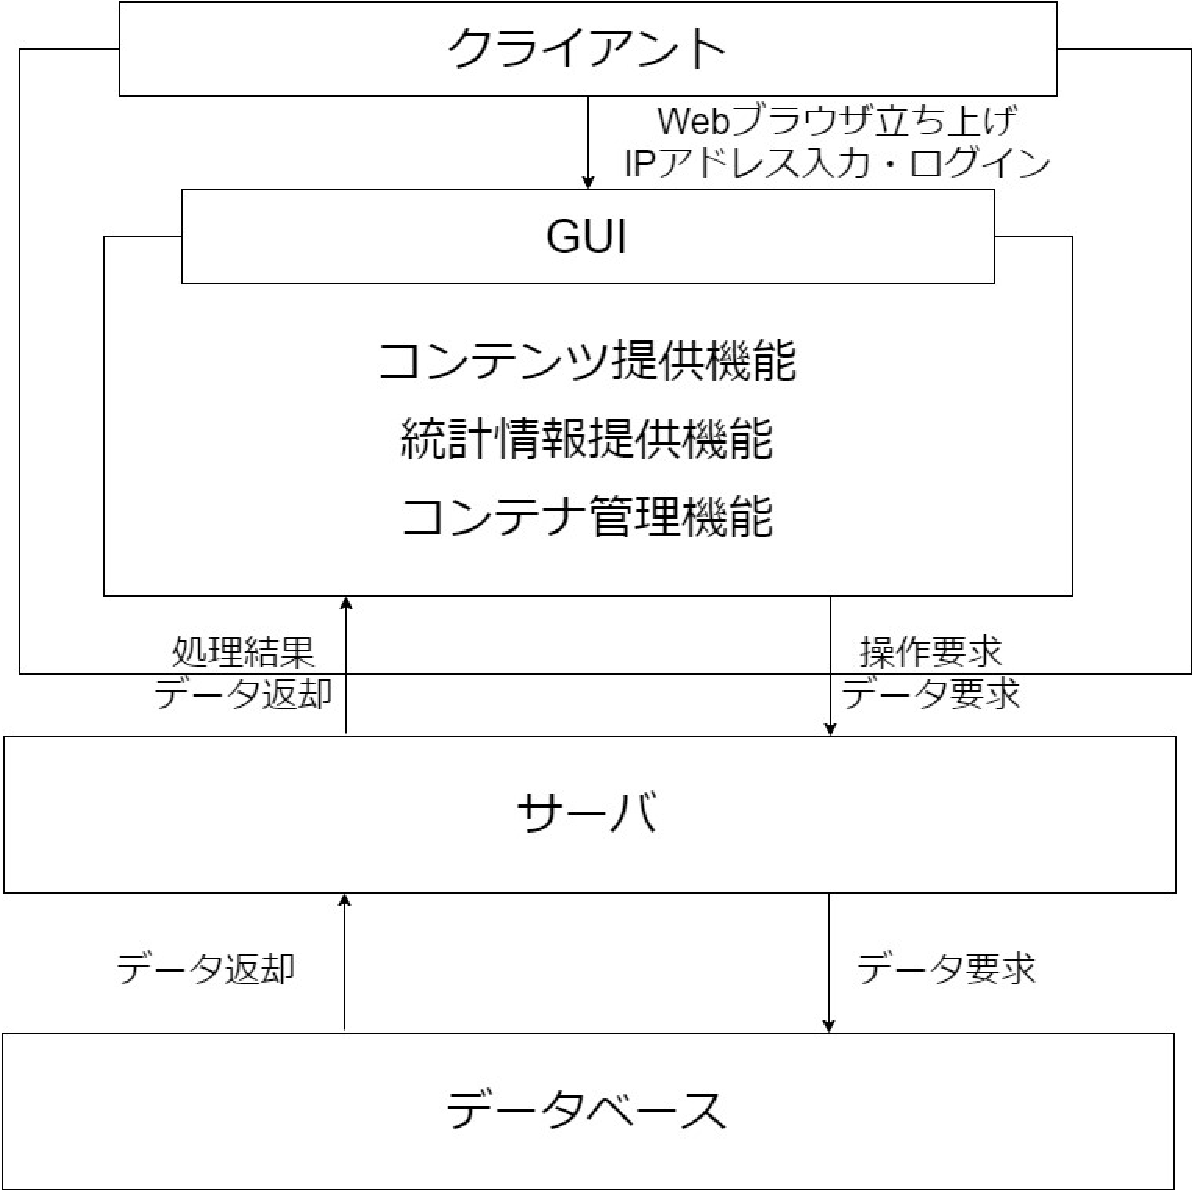
\includegraphics[width=13cm,height=12cm,keepaspectratio]{client_arch-crop.pdf}\\
        %includegraphicsの詳しい使い方ははLaTeXの参考書を参照.
    \end{center}
    \caption{クライアントの内部構成}
    \label{client_naibu}
\end{figure}

\newpage
続いて,サーバの内部構成を図\ref{server_naibu}に示す.サーバはDjangoを用いて作成されたDjango処理部とGoを用いて作成されたGo処理部,データを保存するためのデータベース処理部がある.
サーバはクライアントからの通信が行われた場合に動作する.それぞれの処理部の内容について以下に示す.

\begin{figure}[htbp]
    \begin{center}
        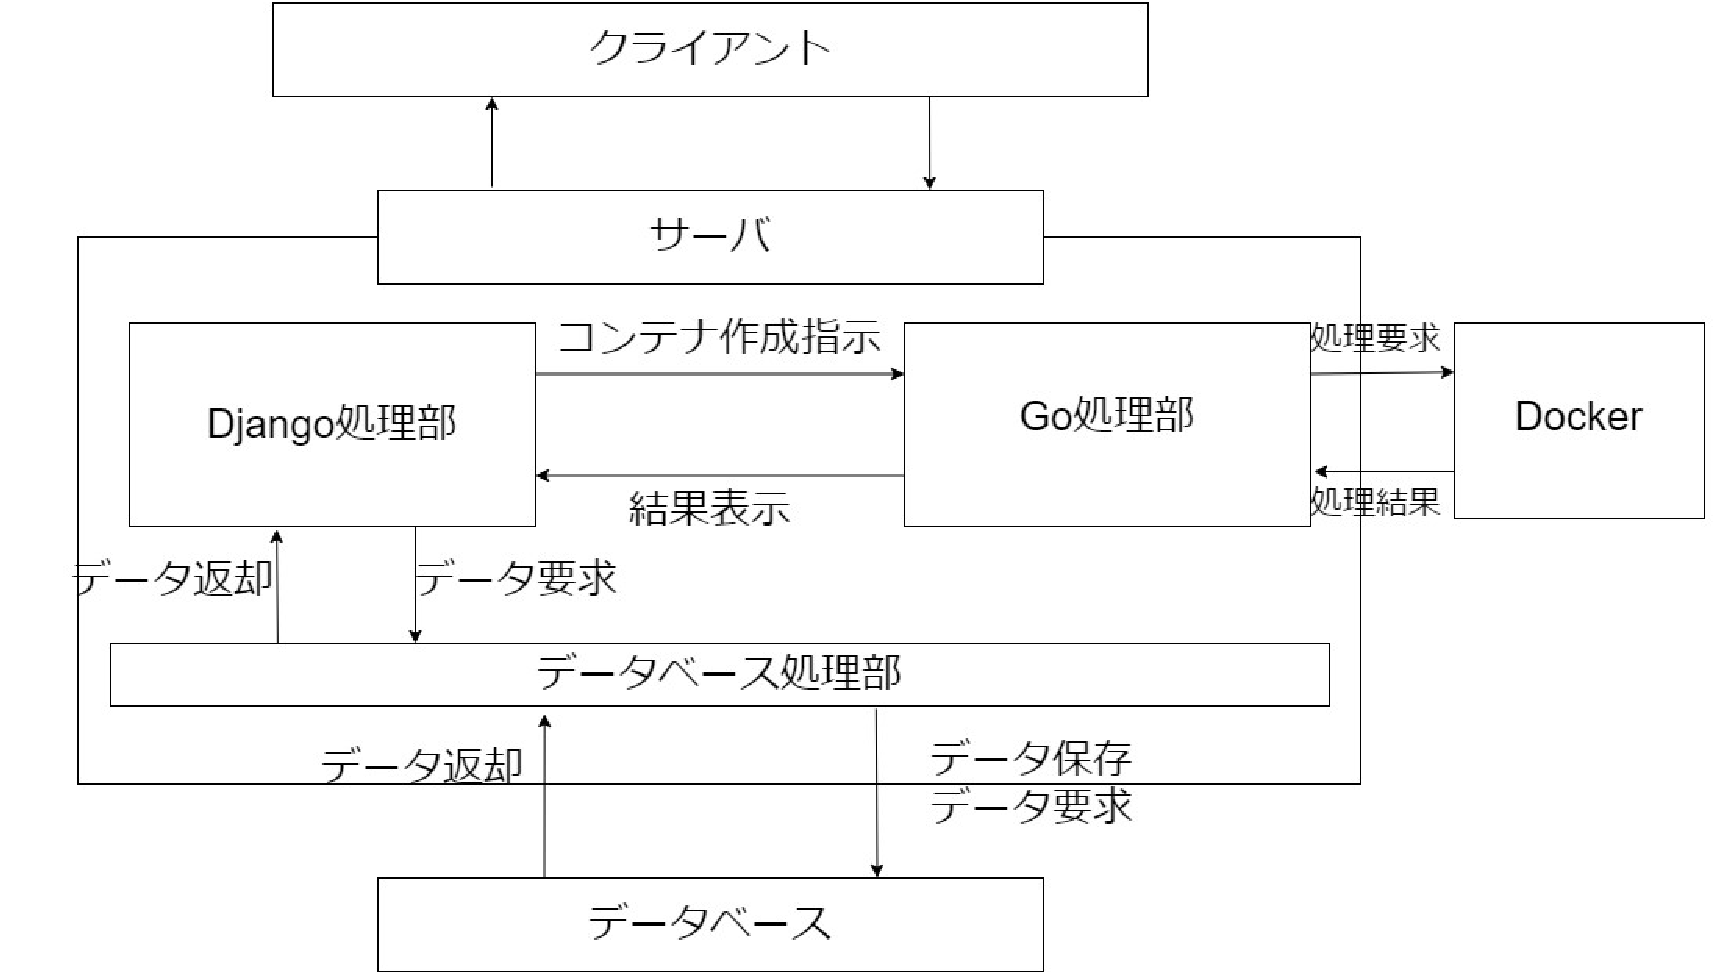
\includegraphics[width=17cm,height=16cm,keepaspectratio]{server_arch-crop.pdf}\\
        %includegraphicsの詳しい使い方ははLaTeXの参考書を参照.
    \end{center}
    \caption{サーバの内部構成}
    \label{server_naibu}
\end{figure}

\begin{description}
    \item[・Django処理部]\mbox{}\\
        Django処理部では,クライアントからフォームに従って入力されたデータをデータベースに登録,抽出する処理を行っている.
        具体的には,ユーザの新規登録,ログイン処理,パスワードや登録情報の変更,コンテンツ提供機能とコンテナ管理機能で入力された情報の登録と修正,タグの検索処理,統計情報提供機能のためのデータの検索が挙げられる.
    \item[・Go処理部]\mbox{}\\
        Go処理部では,コンテナ管理機能により入力された情報をAPIを用いてDockerに実行,処理させコンテナを建ち上げている.
    \item[・データベース処理部]\mbox{}\\
        データベース処理部では,Django処理部においてデータベースのやり取りが必要な場合に動作する.Django処理部からsqlコマンドが発行され,それを実行処理している.
\end{description}

\newpage
\subsubsection{システムのフローチャート}
教材提供者のフローチャートを図\ref{provider_flow}に,学習者のフローチャートを図\ref{learn_flow}に示す.本システムはまず,教材提供者はログインが必須,学習者は任意となっている.そのため今回は簡単のため教材提供者と学習者がともにログインした場合のフローチャートとする.

はじめに教材提供者について説明を行う.教材提供者は事前にユーザ登録を行ったことを管理者に通知し,管理者からアカウントを一般のものから教材提供者のアカウントに設定する必要がある.
教材提供者アカウントに設定した後,ログイン処理を行う.ログインが完了したら教材提供者はコンテンツ提供機能を用いてコンテンツの必要情報を入力し,サーバに対して登録を行う.
統計情報提供機能を用いる場合は,コンテンツに対する統計情報をサーバに対しリクエストすると,その結果が画面上に表示される.
コンテナ管理機能を用いる場合は,動作させたいアプリケーションの情報をクライアント上で入力することにより,サーバに対しその情報がリクエストされ,実行される.実行が正常に完了した場合,接続するためのURLが画面上に表示される.

\begin{figure}[htbp]
    \begin{center}
        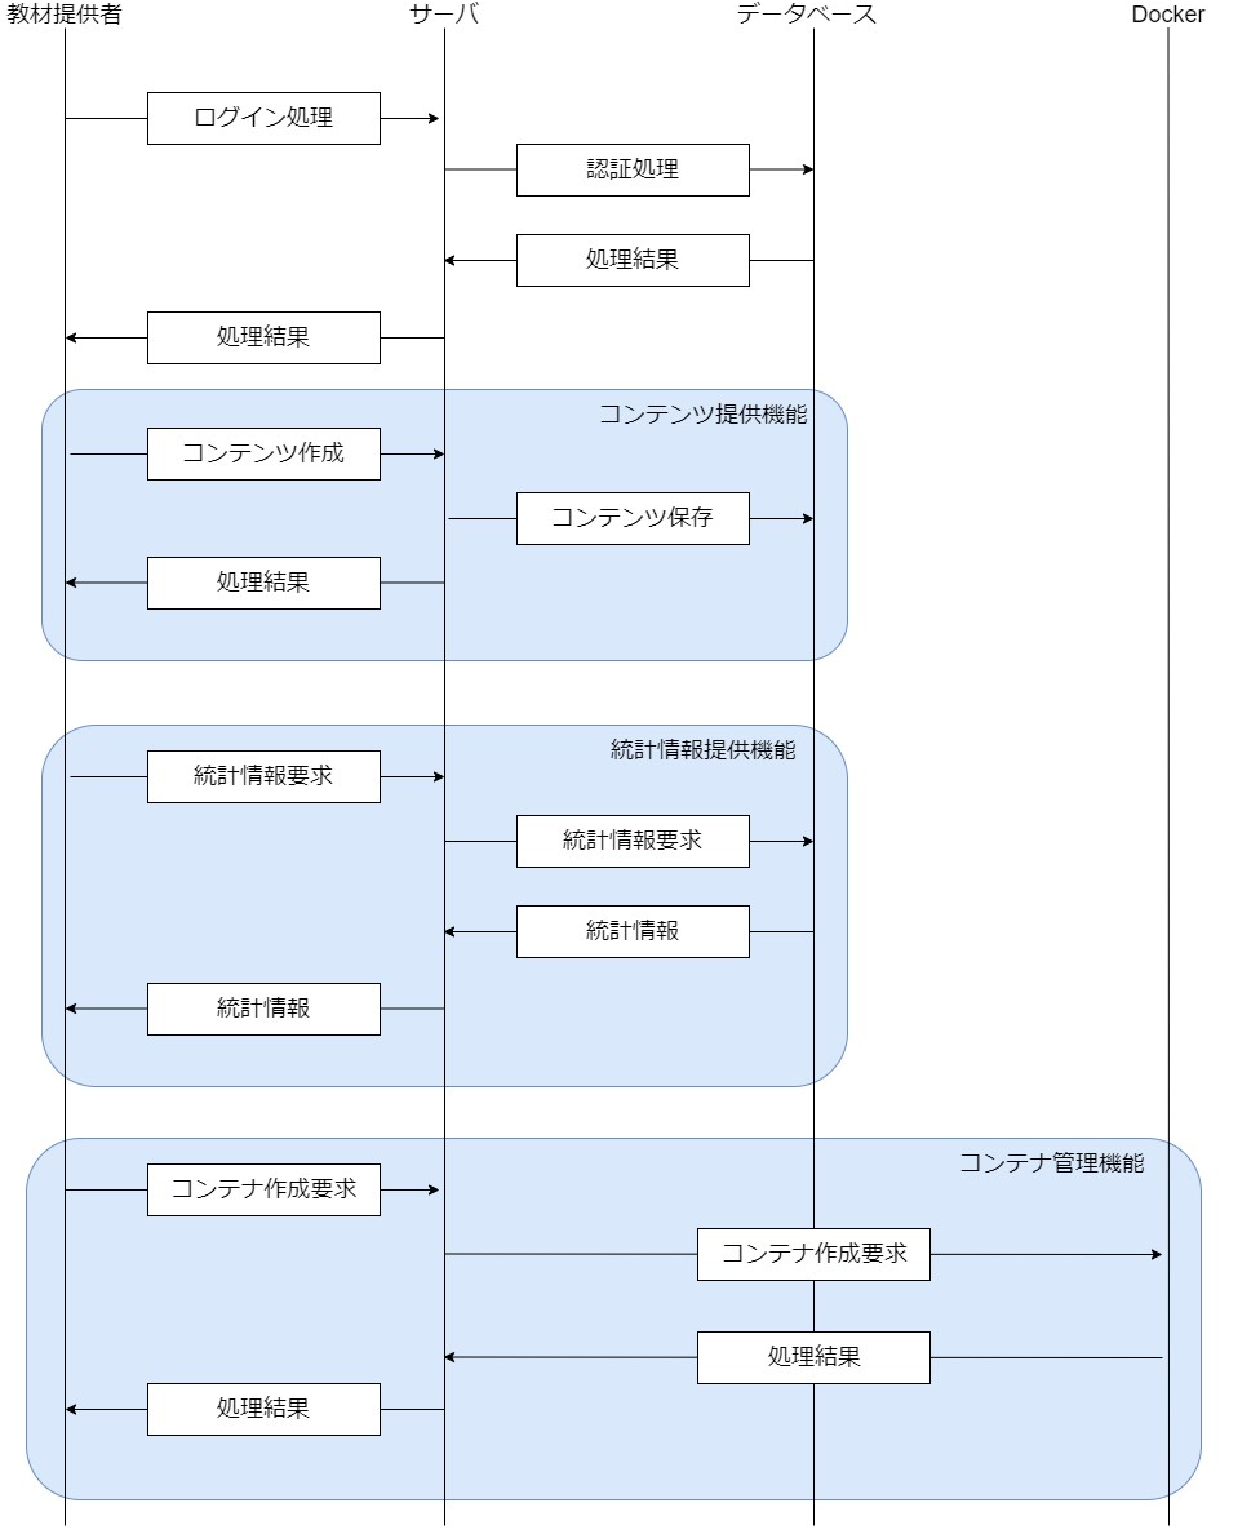
\includegraphics[width=15cm,height=14cm,keepaspectratio]{provider_flow-crop.pdf}\\
        %includegraphicsの詳しい使い方ははLaTeXの参考書を参照.
    \end{center}
    \caption{教材提供者のフローチャート}
    \label{provider_flow}
\end{figure}

\newpage
続いて学習者について説明を行う.学習者はWebブラウザで本プラットフォームに接続した後,本プラットフォームでアカウント作成を行うことができる.アカウント作成には,本プラットフォーム上で表示される
ユーザ名,性別,年齢,パスワードと確認用パスワードが必要である.アカウント作成後,トップページにて教材提供者が作成したコンテンツを選択,閲覧できる.

コンテンツ提供機能,統計情報提供機能,コンテナ管理機能についての詳細は\ref{sec:fun1}節,\ref{sec:fun2}節,\ref{sec:fun3}節にて述べる.

\begin{figure}[htbp]
    \begin{center}
        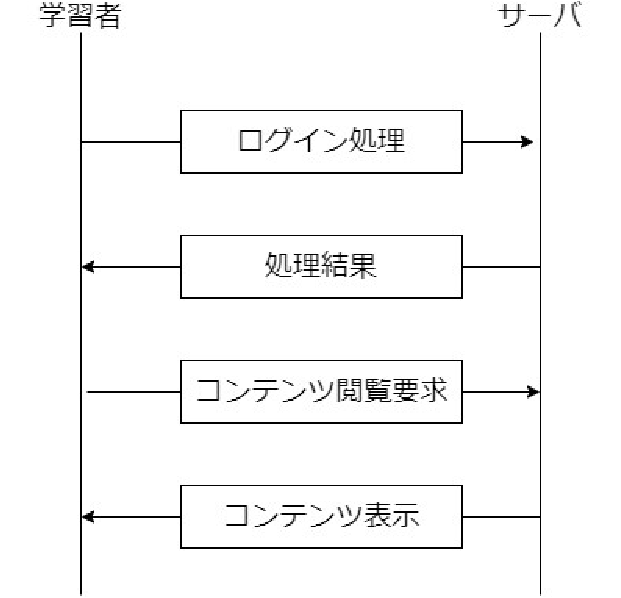
\includegraphics[width=13cm,height=12cm,keepaspectratio]{learn_flow-crop.pdf}\\
        %includegraphicsの詳しい使い方ははLaTeXの参考書を参照.
    \end{center}
    \caption{学習者のフローチャート}
    \label{learn_flow}
\end{figure}